\documentclass[twoside]{book}

% Packages required by doxygen
\usepackage{fixltx2e}
\usepackage{calc}
\usepackage{doxygen}
\usepackage[export]{adjustbox} % also loads graphicx
\usepackage{graphicx}
\usepackage[utf8]{inputenc}
\usepackage{makeidx}
\usepackage{multicol}
\usepackage{multirow}
\PassOptionsToPackage{warn}{textcomp}
\usepackage{textcomp}
\usepackage[nointegrals]{wasysym}
\usepackage[table]{xcolor}

% Font selection
\usepackage[T1]{fontenc}
\usepackage[scaled=.90]{helvet}
\usepackage{courier}
\usepackage{amssymb}
\usepackage{sectsty}
\renewcommand{\familydefault}{\sfdefault}
\allsectionsfont{%
  \fontseries{bc}\selectfont%
  \color{darkgray}%
}
\renewcommand{\DoxyLabelFont}{%
  \fontseries{bc}\selectfont%
  \color{darkgray}%
}
\newcommand{\+}{\discretionary{\mbox{\scriptsize$\hookleftarrow$}}{}{}}

% Page & text layout
\usepackage{geometry}
\geometry{%
  a4paper,%
  top=2.5cm,%
  bottom=2.5cm,%
  left=2.5cm,%
  right=2.5cm%
}
\tolerance=750
\hfuzz=15pt
\hbadness=750
\setlength{\emergencystretch}{15pt}
\setlength{\parindent}{0cm}
\setlength{\parskip}{3ex plus 2ex minus 2ex}
\makeatletter
\renewcommand{\paragraph}{%
  \@startsection{paragraph}{4}{0ex}{-1.0ex}{1.0ex}{%
    \normalfont\normalsize\bfseries\SS@parafont%
  }%
}
\renewcommand{\subparagraph}{%
  \@startsection{subparagraph}{5}{0ex}{-1.0ex}{1.0ex}{%
    \normalfont\normalsize\bfseries\SS@subparafont%
  }%
}
\makeatother

% Headers & footers
\usepackage{fancyhdr}
\pagestyle{fancyplain}
\fancyhead[LE]{\fancyplain{}{\bfseries\thepage}}
\fancyhead[CE]{\fancyplain{}{}}
\fancyhead[RE]{\fancyplain{}{\bfseries\leftmark}}
\fancyhead[LO]{\fancyplain{}{\bfseries\rightmark}}
\fancyhead[CO]{\fancyplain{}{}}
\fancyhead[RO]{\fancyplain{}{\bfseries\thepage}}
\fancyfoot[LE]{\fancyplain{}{}}
\fancyfoot[CE]{\fancyplain{}{}}
\fancyfoot[RE]{\fancyplain{}{\bfseries\scriptsize Generated by Doxygen }}
\fancyfoot[LO]{\fancyplain{}{\bfseries\scriptsize Generated by Doxygen }}
\fancyfoot[CO]{\fancyplain{}{}}
\fancyfoot[RO]{\fancyplain{}{}}
\renewcommand{\footrulewidth}{0.4pt}
\renewcommand{\chaptermark}[1]{%
  \markboth{#1}{}%
}
\renewcommand{\sectionmark}[1]{%
  \markright{\thesection\ #1}%
}

% Indices & bibliography
\usepackage{natbib}
\usepackage[titles]{tocloft}
\setcounter{tocdepth}{3}
\setcounter{secnumdepth}{5}
\makeindex

% Hyperlinks (required, but should be loaded last)
\usepackage{ifpdf}
\ifpdf
  \usepackage[pdftex,pagebackref=true]{hyperref}
\else
  \usepackage[ps2pdf,pagebackref=true]{hyperref}
\fi
\hypersetup{%
  colorlinks=true,%
  linkcolor=blue,%
  citecolor=blue,%
  unicode%
}

% Custom commands
\newcommand{\clearemptydoublepage}{%
  \newpage{\pagestyle{empty}\cleardoublepage}%
}

\usepackage{caption}
\captionsetup{labelsep=space,justification=centering,font={bf},singlelinecheck=off,skip=4pt,position=top}

%===== C O N T E N T S =====

\begin{document}

% Titlepage & ToC
\hypersetup{pageanchor=false,
             bookmarksnumbered=true,
             pdfencoding=unicode
            }
\pagenumbering{alph}
\begin{titlepage}
\vspace*{7cm}
\begin{center}%
{\Large Laboratorio 5 }\\
\vspace*{1cm}
{\large Generated by Doxygen 1.8.12}\\
\end{center}
\end{titlepage}
\clearemptydoublepage
\pagenumbering{roman}
\tableofcontents
\clearemptydoublepage
\pagenumbering{arabic}
\hypersetup{pageanchor=true}

%--- Begin generated contents ---
\chapter{Hierarchical Index}
\section{Class Hierarchy}
This inheritance list is sorted roughly, but not completely, alphabetically\+:\begin{DoxyCompactList}
\item \contentsline{section}{Figuras}{\pageref{class_figuras}}{}
\begin{DoxyCompactList}
\item \contentsline{section}{Circulo}{\pageref{class_circulo}}{}
\item \contentsline{section}{Cuadrado}{\pageref{class_cuadrado}}{}
\item \contentsline{section}{Triangulo}{\pageref{class_triangulo}}{}
\end{DoxyCompactList}
\end{DoxyCompactList}

\chapter{Class Index}
\section{Class List}
Here are the classes, structs, unions and interfaces with brief descriptions\+:\begin{DoxyCompactList}
\item\contentsline{section}{\hyperlink{classblastobject}{blastobject} }{\pageref{classblastobject}}{}
\end{DoxyCompactList}

\chapter{Class Documentation}
\hypertarget{class_lista}{}\section{Lista$<$ T $>$ Class Template Reference}
\label{class_lista}\index{Lista$<$ T $>$@{Lista$<$ T $>$}}


Inheritance diagram for Lista$<$ T $>$\+:
\nopagebreak
\begin{figure}[H]
\begin{center}
\leavevmode
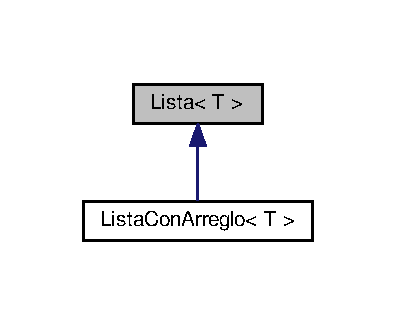
\includegraphics[width=190pt]{class_lista__inherit__graph}
\end{center}
\end{figure}
\subsection*{Public Member Functions}
\begin{DoxyCompactItemize}
\item 
\hypertarget{class_lista_ad63a49df32595e2f321fffd7ffa1346a}{}\label{class_lista_ad63a49df32595e2f321fffd7ffa1346a} 
{\bfseries Lista} (const \hyperlink{class_lista}{Lista} \&orig)
\item 
\hypertarget{class_lista_a1093c2435a3be6d4a74dd75f14ef1428}{}\label{class_lista_a1093c2435a3be6d4a74dd75f14ef1428} 
virtual void {\bfseries agregar} (T const \&e)=0
\item 
\hypertarget{class_lista_a9d459c3698152b71b928e0d9b2d0a318}{}\label{class_lista_a9d459c3698152b71b928e0d9b2d0a318} 
virtual void {\bfseries eliminar} (T const \&e)=0
\item 
\hypertarget{class_lista_aea4b7bb82c177d45fd05b4e98449b45d}{}\label{class_lista_aea4b7bb82c177d45fd05b4e98449b45d} 
virtual void {\bfseries eliminarK} (int k)=0
\item 
\hypertarget{class_lista_ac29cb21fd75a23a34ff7ff517b350b5b}{}\label{class_lista_ac29cb21fd75a23a34ff7ff517b350b5b} 
virtual int {\bfseries buscar} (T const \&e)=0
\item 
\hypertarget{class_lista_a42b835552326bc087ac9b13bdba12262}{}\label{class_lista_a42b835552326bc087ac9b13bdba12262} 
virtual T {\bfseries siguienteK} (int k)=0
\item 
\hypertarget{class_lista_a05bd7ecb7fee94d7203d017899710c3a}{}\label{class_lista_a05bd7ecb7fee94d7203d017899710c3a} 
virtual T {\bfseries anteriorK} (int k)=0
\item 
\hypertarget{class_lista_ace159f98c2e63a7d2f042c9f2bd1e0ed}{}\label{class_lista_ace159f98c2e63a7d2f042c9f2bd1e0ed} 
virtual T {\bfseries recuperar} (int k)=0
\item 
\hypertarget{class_lista_af398229330911af031fc1d89a556a840}{}\label{class_lista_af398229330911af031fc1d89a556a840} 
virtual void {\bfseries imprimir} ()=0
\end{DoxyCompactItemize}


The documentation for this class was generated from the following file\+:\begin{DoxyCompactItemize}
\item 
Lista.\+h\end{DoxyCompactItemize}

\hypertarget{class_lista_con_arreglo}{}\section{Lista\+Con\+Arreglo$<$ T $>$ Class Template Reference}
\label{class_lista_con_arreglo}\index{Lista\+Con\+Arreglo$<$ T $>$@{Lista\+Con\+Arreglo$<$ T $>$}}


Plantilla para construir una \hyperlink{class_lista}{Lista} basada en arreglos.  




{\ttfamily \#include $<$Lista\+Con\+Arreglo.\+h$>$}



Inheritance diagram for Lista\+Con\+Arreglo$<$ T $>$\+:\nopagebreak
\begin{figure}[H]
\begin{center}
\leavevmode
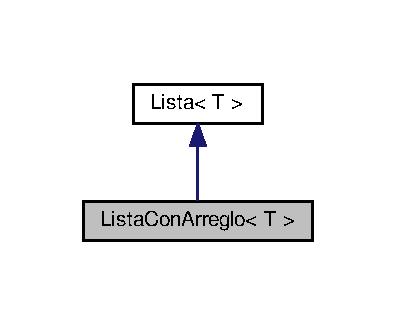
\includegraphics[width=190pt]{class_lista_con_arreglo__inherit__graph}
\end{center}
\end{figure}


Collaboration diagram for Lista\+Con\+Arreglo$<$ T $>$\+:\nopagebreak
\begin{figure}[H]
\begin{center}
\leavevmode
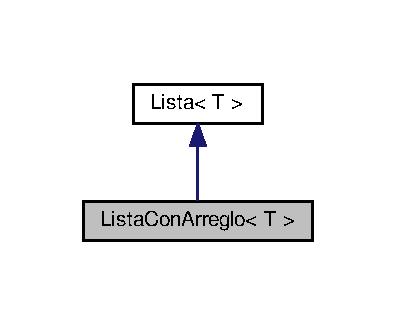
\includegraphics[width=190pt]{class_lista_con_arreglo__coll__graph}
\end{center}
\end{figure}
\subsection*{Public Member Functions}
\begin{DoxyCompactItemize}
\item 
\hypertarget{class_lista_con_arreglo_aeaef142f90f5bea1ecd4121d545f9c73}{}\label{class_lista_con_arreglo_aeaef142f90f5bea1ecd4121d545f9c73} 
\hyperlink{class_lista_con_arreglo_aeaef142f90f5bea1ecd4121d545f9c73}{Lista\+Con\+Arreglo} ()
\begin{DoxyCompactList}\small\item\em Constructor de \hyperlink{class_lista_con_arreglo}{Lista\+Con\+Arreglo}. \end{DoxyCompactList}\item 
\hyperlink{class_lista_con_arreglo_a9541812a0019b76c6529184356913a59}{Lista\+Con\+Arreglo} (int N)
\begin{DoxyCompactList}\small\item\em Constructor sobrecargado de la clase \hyperlink{class_lista_con_arreglo}{Lista\+Con\+Arreglo}. \end{DoxyCompactList}\item 
\hyperlink{class_lista_con_arreglo_ab7a22a8f04de9403d32a7431d4dd9627}{Lista\+Con\+Arreglo} (const \hyperlink{class_lista_con_arreglo}{Lista\+Con\+Arreglo} \&orig)
\begin{DoxyCompactList}\small\item\em Constructor sobrecargado de la clase \hyperlink{class_lista_con_arreglo}{Lista\+Con\+Arreglo}. \end{DoxyCompactList}\item 
\hypertarget{class_lista_con_arreglo_a79115cdeaa5ff1f6e3817b3c201f88a3}{}\label{class_lista_con_arreglo_a79115cdeaa5ff1f6e3817b3c201f88a3} 
\hyperlink{class_lista_con_arreglo_a79115cdeaa5ff1f6e3817b3c201f88a3}{$\sim$\+Lista\+Con\+Arreglo} ()
\begin{DoxyCompactList}\small\item\em Destructor de la clase \hyperlink{class_lista_con_arreglo}{Lista\+Con\+Arreglo}. \end{DoxyCompactList}\item 
void \hyperlink{class_lista_con_arreglo_a0164c47d0fb79d355a30f9b7acd8c762}{agregar} (const T \&e)
\begin{DoxyCompactList}\small\item\em Agrega un elemento. \end{DoxyCompactList}\item 
void \hyperlink{class_lista_con_arreglo_abff25d43f812199b55bb34df9084c9ac}{sumark} (int k, const T \&e)
\begin{DoxyCompactList}\small\item\em Suma un elemento. \end{DoxyCompactList}\item 
void \hyperlink{class_lista_con_arreglo_a742afe90aa461d9dafbf9579c6615c81}{agregark} (int k, const T \&e)
\begin{DoxyCompactList}\small\item\em Agrega en una posicion un elemento. \end{DoxyCompactList}\item 
void \hyperlink{class_lista_con_arreglo_a0ee68c7b0f66324764bacd4ee4ffab50}{eliminar} (const T \&e)
\begin{DoxyCompactList}\small\item\em Elimina un elemento. \end{DoxyCompactList}\item 
void \hyperlink{class_lista_con_arreglo_acd8b8f484dc440dc64dc58cad375e7e4}{eliminarK} (int k)
\begin{DoxyCompactList}\small\item\em Elimina una posicion. \end{DoxyCompactList}\item 
int \hyperlink{class_lista_con_arreglo_a93187f91395bd4a498624470524a40aa}{buscar} (const T \&e)
\begin{DoxyCompactList}\small\item\em Busca un elemento. \end{DoxyCompactList}\item 
\hypertarget{class_lista_con_arreglo_ad491d37617d43b24c91021db0102fc88}{}\label{class_lista_con_arreglo_ad491d37617d43b24c91021db0102fc88} 
T {\bfseries siguienteK} (int k)
\item 
\hypertarget{class_lista_con_arreglo_ad32acb0a906dafff65201dbb506b48f7}{}\label{class_lista_con_arreglo_ad32acb0a906dafff65201dbb506b48f7} 
T {\bfseries anteriorK} (int k)
\item 
\hypertarget{class_lista_con_arreglo_af880c9a6795cf9281f2a217d0a4b0c07}{}\label{class_lista_con_arreglo_af880c9a6795cf9281f2a217d0a4b0c07} 
T {\bfseries recuperar} (int k)
\item 
\hypertarget{class_lista_con_arreglo_aa8267cef7510ef79626a812b3c85505d}{}\label{class_lista_con_arreglo_aa8267cef7510ef79626a812b3c85505d} 
void \hyperlink{class_lista_con_arreglo_aa8267cef7510ef79626a812b3c85505d}{imprimir} ()
\begin{DoxyCompactList}\small\item\em Imprime la lista. \end{DoxyCompactList}\item 
\hypertarget{class_lista_con_arreglo_ad66ab536ce3bdf4df20ee7e89cd148ee}{}\label{class_lista_con_arreglo_ad66ab536ce3bdf4df20ee7e89cd148ee} 
bool {\bfseries vacio} ()
\end{DoxyCompactItemize}
\subsection*{Public Attributes}
\begin{DoxyCompactItemize}
\item 
\hypertarget{class_lista_con_arreglo_a7b1a9c6334db75f4ffb023a95b01e3f4}{}\label{class_lista_con_arreglo_a7b1a9c6334db75f4ffb023a95b01e3f4} 
int {\bfseries tam} = 0
\end{DoxyCompactItemize}


\subsection{Detailed Description}
\subsubsection*{template$<$class T$>$\\*
class Lista\+Con\+Arreglo$<$ T $>$}

Plantilla para construir una \hyperlink{class_lista}{Lista} basada en arreglos. 

\subsection{Constructor \& Destructor Documentation}
\hypertarget{class_lista_con_arreglo_a9541812a0019b76c6529184356913a59}{}\label{class_lista_con_arreglo_a9541812a0019b76c6529184356913a59} 
\index{Lista\+Con\+Arreglo@{Lista\+Con\+Arreglo}!Lista\+Con\+Arreglo@{Lista\+Con\+Arreglo}}
\index{Lista\+Con\+Arreglo@{Lista\+Con\+Arreglo}!Lista\+Con\+Arreglo@{Lista\+Con\+Arreglo}}
\subsubsection{\texorpdfstring{Lista\+Con\+Arreglo()}{ListaConArreglo()}\hspace{0.1cm}{\footnotesize\ttfamily [1/2]}}
{\ttfamily template$<$class T$>$ \\
\hyperlink{class_lista_con_arreglo}{Lista\+Con\+Arreglo}$<$ T $>$\+::\hyperlink{class_lista_con_arreglo}{Lista\+Con\+Arreglo} (\begin{DoxyParamCaption}\item[{int}]{N }\end{DoxyParamCaption})\hspace{0.3cm}{\ttfamily [inline]}}



Constructor sobrecargado de la clase \hyperlink{class_lista_con_arreglo}{Lista\+Con\+Arreglo}. 


\begin{DoxyParams}{Parameters}
{\em N} & Dimension de \hyperlink{class_lista}{Lista}. \\
\hline
\end{DoxyParams}
\hypertarget{class_lista_con_arreglo_ab7a22a8f04de9403d32a7431d4dd9627}{}\label{class_lista_con_arreglo_ab7a22a8f04de9403d32a7431d4dd9627} 
\index{Lista\+Con\+Arreglo@{Lista\+Con\+Arreglo}!Lista\+Con\+Arreglo@{Lista\+Con\+Arreglo}}
\index{Lista\+Con\+Arreglo@{Lista\+Con\+Arreglo}!Lista\+Con\+Arreglo@{Lista\+Con\+Arreglo}}
\subsubsection{\texorpdfstring{Lista\+Con\+Arreglo()}{ListaConArreglo()}\hspace{0.1cm}{\footnotesize\ttfamily [2/2]}}
{\ttfamily template$<$class T$>$ \\
\hyperlink{class_lista_con_arreglo}{Lista\+Con\+Arreglo}$<$ T $>$\+::\hyperlink{class_lista_con_arreglo}{Lista\+Con\+Arreglo} (\begin{DoxyParamCaption}\item[{const \hyperlink{class_lista_con_arreglo}{Lista\+Con\+Arreglo}$<$ T $>$ \&}]{orig }\end{DoxyParamCaption})\hspace{0.3cm}{\ttfamily [inline]}}



Constructor sobrecargado de la clase \hyperlink{class_lista_con_arreglo}{Lista\+Con\+Arreglo}. 


\begin{DoxyParams}{Parameters}
{\em Lista\+Con\+Arreglo\&} & Objeto del tipo \hyperlink{class_lista_con_arreglo}{Lista\+Con\+Arreglo}. \\
\hline
\end{DoxyParams}


\subsection{Member Function Documentation}
\hypertarget{class_lista_con_arreglo_a0164c47d0fb79d355a30f9b7acd8c762}{}\label{class_lista_con_arreglo_a0164c47d0fb79d355a30f9b7acd8c762} 
\index{Lista\+Con\+Arreglo@{Lista\+Con\+Arreglo}!agregar@{agregar}}
\index{agregar@{agregar}!Lista\+Con\+Arreglo@{Lista\+Con\+Arreglo}}
\subsubsection{\texorpdfstring{agregar()}{agregar()}}
{\ttfamily template$<$class T$>$ \\
void \hyperlink{class_lista_con_arreglo}{Lista\+Con\+Arreglo}$<$ T $>$\+::agregar (\begin{DoxyParamCaption}\item[{const T \&}]{e }\end{DoxyParamCaption})\hspace{0.3cm}{\ttfamily [inline]}, {\ttfamily [virtual]}}



Agrega un elemento. 


\begin{DoxyParams}{Parameters}
{\em \&e} & Elemento por agregar. \\
\hline
\end{DoxyParams}


Implements \hyperlink{class_lista}{Lista$<$ T $>$}.

\hypertarget{class_lista_con_arreglo_a742afe90aa461d9dafbf9579c6615c81}{}\label{class_lista_con_arreglo_a742afe90aa461d9dafbf9579c6615c81} 
\index{Lista\+Con\+Arreglo@{Lista\+Con\+Arreglo}!agregark@{agregark}}
\index{agregark@{agregark}!Lista\+Con\+Arreglo@{Lista\+Con\+Arreglo}}
\subsubsection{\texorpdfstring{agregark()}{agregark()}}
{\ttfamily template$<$class T$>$ \\
void \hyperlink{class_lista_con_arreglo}{Lista\+Con\+Arreglo}$<$ T $>$\+::agregark (\begin{DoxyParamCaption}\item[{int}]{k,  }\item[{const T \&}]{e }\end{DoxyParamCaption})\hspace{0.3cm}{\ttfamily [inline]}}



Agrega en una posicion un elemento. 


\begin{DoxyParams}{Parameters}
{\em k} & Posicion. \\
\hline
{\em \&e} & Elemento por agregar. \\
\hline
\end{DoxyParams}
\hypertarget{class_lista_con_arreglo_a93187f91395bd4a498624470524a40aa}{}\label{class_lista_con_arreglo_a93187f91395bd4a498624470524a40aa} 
\index{Lista\+Con\+Arreglo@{Lista\+Con\+Arreglo}!buscar@{buscar}}
\index{buscar@{buscar}!Lista\+Con\+Arreglo@{Lista\+Con\+Arreglo}}
\subsubsection{\texorpdfstring{buscar()}{buscar()}}
{\ttfamily template$<$class T$>$ \\
int \hyperlink{class_lista_con_arreglo}{Lista\+Con\+Arreglo}$<$ T $>$\+::buscar (\begin{DoxyParamCaption}\item[{const T \&}]{e }\end{DoxyParamCaption})\hspace{0.3cm}{\ttfamily [inline]}, {\ttfamily [virtual]}}



Busca un elemento. 


\begin{DoxyParams}{Parameters}
{\em \&e} & Elemento por buscar. \\
\hline
\end{DoxyParams}


Implements \hyperlink{class_lista}{Lista$<$ T $>$}.

\hypertarget{class_lista_con_arreglo_a0ee68c7b0f66324764bacd4ee4ffab50}{}\label{class_lista_con_arreglo_a0ee68c7b0f66324764bacd4ee4ffab50} 
\index{Lista\+Con\+Arreglo@{Lista\+Con\+Arreglo}!eliminar@{eliminar}}
\index{eliminar@{eliminar}!Lista\+Con\+Arreglo@{Lista\+Con\+Arreglo}}
\subsubsection{\texorpdfstring{eliminar()}{eliminar()}}
{\ttfamily template$<$class T$>$ \\
void \hyperlink{class_lista_con_arreglo}{Lista\+Con\+Arreglo}$<$ T $>$\+::eliminar (\begin{DoxyParamCaption}\item[{const T \&}]{e }\end{DoxyParamCaption})\hspace{0.3cm}{\ttfamily [inline]}, {\ttfamily [virtual]}}



Elimina un elemento. 


\begin{DoxyParams}{Parameters}
{\em \&e} & Elemento por eliminar \\
\hline
\end{DoxyParams}


Implements \hyperlink{class_lista}{Lista$<$ T $>$}.

\hypertarget{class_lista_con_arreglo_acd8b8f484dc440dc64dc58cad375e7e4}{}\label{class_lista_con_arreglo_acd8b8f484dc440dc64dc58cad375e7e4} 
\index{Lista\+Con\+Arreglo@{Lista\+Con\+Arreglo}!eliminarK@{eliminarK}}
\index{eliminarK@{eliminarK}!Lista\+Con\+Arreglo@{Lista\+Con\+Arreglo}}
\subsubsection{\texorpdfstring{eliminar\+K()}{eliminarK()}}
{\ttfamily template$<$class T$>$ \\
void \hyperlink{class_lista_con_arreglo}{Lista\+Con\+Arreglo}$<$ T $>$\+::eliminarK (\begin{DoxyParamCaption}\item[{int}]{k }\end{DoxyParamCaption})\hspace{0.3cm}{\ttfamily [inline]}, {\ttfamily [virtual]}}



Elimina una posicion. 


\begin{DoxyParams}{Parameters}
{\em k} & Posicion. \\
\hline
\end{DoxyParams}


Implements \hyperlink{class_lista}{Lista$<$ T $>$}.

\hypertarget{class_lista_con_arreglo_abff25d43f812199b55bb34df9084c9ac}{}\label{class_lista_con_arreglo_abff25d43f812199b55bb34df9084c9ac} 
\index{Lista\+Con\+Arreglo@{Lista\+Con\+Arreglo}!sumark@{sumark}}
\index{sumark@{sumark}!Lista\+Con\+Arreglo@{Lista\+Con\+Arreglo}}
\subsubsection{\texorpdfstring{sumark()}{sumark()}}
{\ttfamily template$<$class T$>$ \\
void \hyperlink{class_lista_con_arreglo}{Lista\+Con\+Arreglo}$<$ T $>$\+::sumark (\begin{DoxyParamCaption}\item[{int}]{k,  }\item[{const T \&}]{e }\end{DoxyParamCaption})\hspace{0.3cm}{\ttfamily [inline]}}



Suma un elemento. 


\begin{DoxyParams}{Parameters}
{\em k} & Elemento al cual sumar. \\
\hline
{\em \&e} & Elemento por sumar \\
\hline
\end{DoxyParams}


The documentation for this class was generated from the following file\+:\begin{DoxyCompactItemize}
\item 
Lista\+Con\+Arreglo.\+h\end{DoxyCompactItemize}

\hypertarget{class_mesa}{}\section{Mesa Class Reference}
\label{class_mesa}\index{Mesa@{Mesa}}


Collaboration diagram for Mesa\+:\nopagebreak
\begin{figure}[H]
\begin{center}
\leavevmode
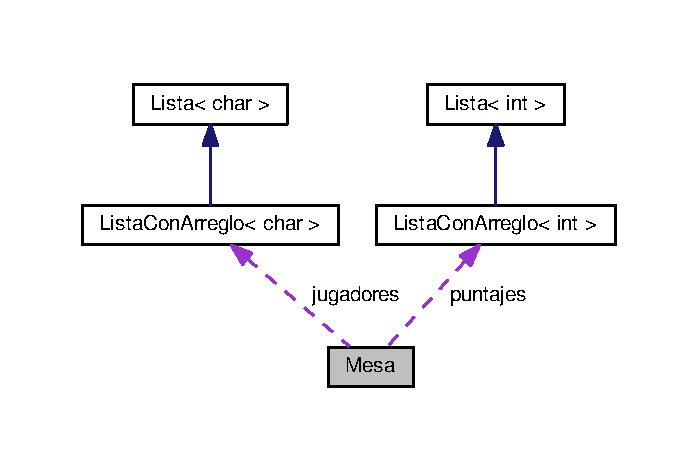
\includegraphics[width=335pt]{class_mesa__coll__graph}
\end{center}
\end{figure}
\subsection*{Public Member Functions}
\begin{DoxyCompactItemize}
\item 
\hypertarget{class_mesa_a98794038db53804cb4295480c96b2c20}{}\label{class_mesa_a98794038db53804cb4295480c96b2c20} 
\hyperlink{class_mesa_a98794038db53804cb4295480c96b2c20}{Mesa} ()
\begin{DoxyCompactList}\small\item\em Constructor de clase \hyperlink{class_mesa}{Mesa}. \end{DoxyCompactList}\item 
\hyperlink{class_mesa_a8cb7a7932e52b13242eaa5ade9f646cb}{Mesa} (int N)
\begin{DoxyCompactList}\small\item\em Constructor de clase \hyperlink{class_mesa}{Mesa} sobrecargado. \end{DoxyCompactList}\item 
\hyperlink{class_mesa_af28f64b3a29b75d2a281dbc1d439a74e}{Mesa} (const \hyperlink{class_mesa}{Mesa} \&orig)
\begin{DoxyCompactList}\small\item\em Imprime una cadena de caracteres dada por el usuario. \end{DoxyCompactList}\item 
\hypertarget{class_mesa_aa0a1b83b8058f80f4f27ec46cc5e9524}{}\label{class_mesa_aa0a1b83b8058f80f4f27ec46cc5e9524} 
virtual \hyperlink{class_mesa_aa0a1b83b8058f80f4f27ec46cc5e9524}{$\sim$\+Mesa} ()
\begin{DoxyCompactList}\small\item\em Destructor de la clase \hyperlink{class_mesa}{Mesa}. \end{DoxyCompactList}\item 
void \hyperlink{class_mesa_a567e239c0dedc7d2aadb0633b4f1580b}{Blackjack} (\hyperlink{class_lista_con_arreglo}{Lista\+Con\+Arreglo}$<$ char $>$ $\ast$admision)
\begin{DoxyCompactList}\small\item\em Funcion principal de distribucion para el juego de Blackjack. \end{DoxyCompactList}\item 
void \hyperlink{class_mesa_ad8160d20365c5d6e8434e2ebd2c75b06}{agregar\+\_\+jugador} (\hyperlink{class_lista_con_arreglo}{Lista\+Con\+Arreglo}$<$ char $>$ $\ast$admision)
\begin{DoxyCompactList}\small\item\em Agrega jugador a la mesa de juego. \end{DoxyCompactList}\item 
void \hyperlink{class_mesa_a6b366909106ac813211e0e36703dc1b1}{sacar\+\_\+jugador} (int i)
\begin{DoxyCompactList}\small\item\em Elimina jugador a la mesa de juego. \end{DoxyCompactList}\item 
\hypertarget{class_mesa_a35761c94c89ffcd57873b981428391db}{}\label{class_mesa_a35761c94c89ffcd57873b981428391db} 
void \hyperlink{class_mesa_a35761c94c89ffcd57873b981428391db}{barajar} ()
\begin{DoxyCompactList}\small\item\em Prepara las cartas para el juego. \end{DoxyCompactList}\item 
\hypertarget{class_mesa_a67c92e9165893fcdb496f37fae7fe30c}{}\label{class_mesa_a67c92e9165893fcdb496f37fae7fe30c} 
bool \hyperlink{class_mesa_a67c92e9165893fcdb496f37fae7fe30c}{lleno} ()
\begin{DoxyCompactList}\small\item\em Revisa si la mesa esta llena o no. \end{DoxyCompactList}\item 
void \hyperlink{class_mesa_a1aafcc25c473a282495a4c7043fb42de}{llenar} (\hyperlink{class_lista_con_arreglo}{Lista\+Con\+Arreglo}$<$ char $>$ $\ast$Admision)
\begin{DoxyCompactList}\small\item\em Llena las mesas para el juego. \end{DoxyCompactList}\item 
\hypertarget{class_mesa_ac7098158c1fcdf3846494d65b5ff6f06}{}\label{class_mesa_ac7098158c1fcdf3846494d65b5ff6f06} 
void \hyperlink{class_mesa_ac7098158c1fcdf3846494d65b5ff6f06}{vaciar} ()
\begin{DoxyCompactList}\small\item\em Vacia la mesa. \end{DoxyCompactList}\end{DoxyCompactItemize}
\subsection*{Public Attributes}
\begin{DoxyCompactItemize}
\item 
\hypertarget{class_mesa_a7ccf2ba385f9a7b167b7f262ed1b1d91}{}\label{class_mesa_a7ccf2ba385f9a7b167b7f262ed1b1d91} 
\hyperlink{class_lista_con_arreglo}{Lista\+Con\+Arreglo}$<$ char $>$ $\ast$ {\bfseries jugadores}
\item 
\hypertarget{class_mesa_af3babe5df4e164206cf5c32138fb3516}{}\label{class_mesa_af3babe5df4e164206cf5c32138fb3516} 
\hyperlink{class_lista_con_arreglo}{Lista\+Con\+Arreglo}$<$ int $>$ $\ast$ {\bfseries puntajes}
\item 
\hypertarget{class_mesa_a1fc67802b221fd42d6a979c2bfc4833d}{}\label{class_mesa_a1fc67802b221fd42d6a979c2bfc4833d} 
int {\bfseries ronda}
\end{DoxyCompactItemize}


\subsection{Constructor \& Destructor Documentation}
\hypertarget{class_mesa_a8cb7a7932e52b13242eaa5ade9f646cb}{}\label{class_mesa_a8cb7a7932e52b13242eaa5ade9f646cb} 
\index{Mesa@{Mesa}!Mesa@{Mesa}}
\index{Mesa@{Mesa}!Mesa@{Mesa}}
\subsubsection{\texorpdfstring{Mesa()}{Mesa()}\hspace{0.1cm}{\footnotesize\ttfamily [1/2]}}
{\ttfamily Mesa\+::\+Mesa (\begin{DoxyParamCaption}\item[{int}]{N }\end{DoxyParamCaption})}



Constructor de clase \hyperlink{class_mesa}{Mesa} sobrecargado. 


\begin{DoxyParams}{Parameters}
{\em N} & dimension del arreglo. \\
\hline
\end{DoxyParams}
\hypertarget{class_mesa_af28f64b3a29b75d2a281dbc1d439a74e}{}\label{class_mesa_af28f64b3a29b75d2a281dbc1d439a74e} 
\index{Mesa@{Mesa}!Mesa@{Mesa}}
\index{Mesa@{Mesa}!Mesa@{Mesa}}
\subsubsection{\texorpdfstring{Mesa()}{Mesa()}\hspace{0.1cm}{\footnotesize\ttfamily [2/2]}}
{\ttfamily Mesa\+::\+Mesa (\begin{DoxyParamCaption}\item[{const \hyperlink{class_mesa}{Mesa} \&}]{orig }\end{DoxyParamCaption})}



Imprime una cadena de caracteres dada por el usuario. 


\begin{DoxyParams}{Parameters}
{\em Mesa\&} & Objeto del tipo \hyperlink{class_mesa}{Mesa}. \\
\hline
\end{DoxyParams}


\subsection{Member Function Documentation}
\hypertarget{class_mesa_ad8160d20365c5d6e8434e2ebd2c75b06}{}\label{class_mesa_ad8160d20365c5d6e8434e2ebd2c75b06} 
\index{Mesa@{Mesa}!agregar\+\_\+jugador@{agregar\+\_\+jugador}}
\index{agregar\+\_\+jugador@{agregar\+\_\+jugador}!Mesa@{Mesa}}
\subsubsection{\texorpdfstring{agregar\+\_\+jugador()}{agregar\_jugador()}}
{\ttfamily void Mesa\+::agregar\+\_\+jugador (\begin{DoxyParamCaption}\item[{\hyperlink{class_lista_con_arreglo}{Lista\+Con\+Arreglo}$<$ char $>$ $\ast$}]{admision }\end{DoxyParamCaption})}



Agrega jugador a la mesa de juego. 


\begin{DoxyParams}{Parameters}
{\em Admision} & \hyperlink{class_lista}{Lista} de personas por entrar al juego. \\
\hline
\end{DoxyParams}
\hypertarget{class_mesa_a567e239c0dedc7d2aadb0633b4f1580b}{}\label{class_mesa_a567e239c0dedc7d2aadb0633b4f1580b} 
\index{Mesa@{Mesa}!Blackjack@{Blackjack}}
\index{Blackjack@{Blackjack}!Mesa@{Mesa}}
\subsubsection{\texorpdfstring{Blackjack()}{Blackjack()}}
{\ttfamily void Mesa\+::\+Blackjack (\begin{DoxyParamCaption}\item[{\hyperlink{class_lista_con_arreglo}{Lista\+Con\+Arreglo}$<$ char $>$ $\ast$}]{Admision }\end{DoxyParamCaption})}



Funcion principal de distribucion para el juego de Blackjack. 


\begin{DoxyParams}{Parameters}
{\em Admision} & \hyperlink{class_lista}{Lista} de personas por entrar al juego. \\
\hline
\end{DoxyParams}
\hypertarget{class_mesa_a1aafcc25c473a282495a4c7043fb42de}{}\label{class_mesa_a1aafcc25c473a282495a4c7043fb42de} 
\index{Mesa@{Mesa}!llenar@{llenar}}
\index{llenar@{llenar}!Mesa@{Mesa}}
\subsubsection{\texorpdfstring{llenar()}{llenar()}}
{\ttfamily void Mesa\+::llenar (\begin{DoxyParamCaption}\item[{\hyperlink{class_lista_con_arreglo}{Lista\+Con\+Arreglo}$<$ char $>$ $\ast$}]{Admision }\end{DoxyParamCaption})}



Llena las mesas para el juego. 


\begin{DoxyParams}{Parameters}
{\em Admision} & \hyperlink{class_lista}{Lista} de personas por entrar al juego. \\
\hline
\end{DoxyParams}
\hypertarget{class_mesa_a6b366909106ac813211e0e36703dc1b1}{}\label{class_mesa_a6b366909106ac813211e0e36703dc1b1} 
\index{Mesa@{Mesa}!sacar\+\_\+jugador@{sacar\+\_\+jugador}}
\index{sacar\+\_\+jugador@{sacar\+\_\+jugador}!Mesa@{Mesa}}
\subsubsection{\texorpdfstring{sacar\+\_\+jugador()}{sacar\_jugador()}}
{\ttfamily void Mesa\+::sacar\+\_\+jugador (\begin{DoxyParamCaption}\item[{int}]{i }\end{DoxyParamCaption})}



Elimina jugador a la mesa de juego. 


\begin{DoxyParams}{Parameters}
{\em i} & Orden del jugador. \\
\hline
\end{DoxyParams}


The documentation for this class was generated from the following files\+:\begin{DoxyCompactItemize}
\item 
Mesa.\+h\item 
Mesa.\+cpp\end{DoxyCompactItemize}

\hypertarget{class_pila}{}\section{Pila$<$ T $>$ Class Template Reference}
\label{class_pila}\index{Pila$<$ T $>$@{Pila$<$ T $>$}}
\subsection*{Public Member Functions}
\begin{DoxyCompactItemize}
\item 
\hypertarget{class_pila_a97d428515745369086aecf513990fa24}{}\label{class_pila_a97d428515745369086aecf513990fa24} 
{\bfseries Pila} (int N)
\item 
\hypertarget{class_pila_a88e3da02e61f188d098f77875c221666}{}\label{class_pila_a88e3da02e61f188d098f77875c221666} 
{\bfseries Pila} (const \hyperlink{class_pila}{Pila} \&orig)
\item 
\hypertarget{class_pila_a9250ad4ed594b141d6cdeacc6684ff9a}{}\label{class_pila_a9250ad4ed594b141d6cdeacc6684ff9a} 
T {\bfseries pop} ()
\item 
\hypertarget{class_pila_abec1671867c1881a53fd67a56352e4ba}{}\label{class_pila_abec1671867c1881a53fd67a56352e4ba} 
void {\bfseries push} (T const \&e)
\item 
\hypertarget{class_pila_ad4b5111ccfdb49689ced1af2ba082e52}{}\label{class_pila_ad4b5111ccfdb49689ced1af2ba082e52} 
void {\bfseries imprimir} ()
\item 
\hypertarget{class_pila_a9d5607a089b2ac1b695fe4c251a375fa}{}\label{class_pila_a9d5607a089b2ac1b695fe4c251a375fa} 
void {\bfseries aleatorizar} ()
\item 
\hypertarget{class_pila_a10d685c3878026c0e7ede6c26c193832}{}\label{class_pila_a10d685c3878026c0e7ede6c26c193832} 
bool {\bfseries vacio} ()
\end{DoxyCompactItemize}


The documentation for this class was generated from the following file\+:\begin{DoxyCompactItemize}
\item 
Pila.\+h\end{DoxyCompactItemize}

%--- End generated contents ---

% Index
\backmatter
\newpage
\phantomsection
\clearemptydoublepage
\addcontentsline{toc}{chapter}{Index}
\printindex

\end{document}
